\documentclass[mathserif, 10pt, aspectratio=169]{beamer}
\usepackage[utf8]{inputenc}
\usepackage{amsmath, amsfonts}
\usepackage{appendixnumberbeamer}


\title{Light New Physics in $\tau$}
\subtitle{{\bf JA}, G. Levati, P. Paradisi, S. Rigolin, N. Selimovic}
\author[Jorge Alda]{Jorge Alda \hspace{4em} \texttt{jorge.alda@pd.infn.it} \\
Università degli Studi di Padova \& CAPA}
\date{Saturnalia '23 \\ \today}



\usetheme{Zaragoza}
\usecolortheme{Unipd}
\titlepagelogoA{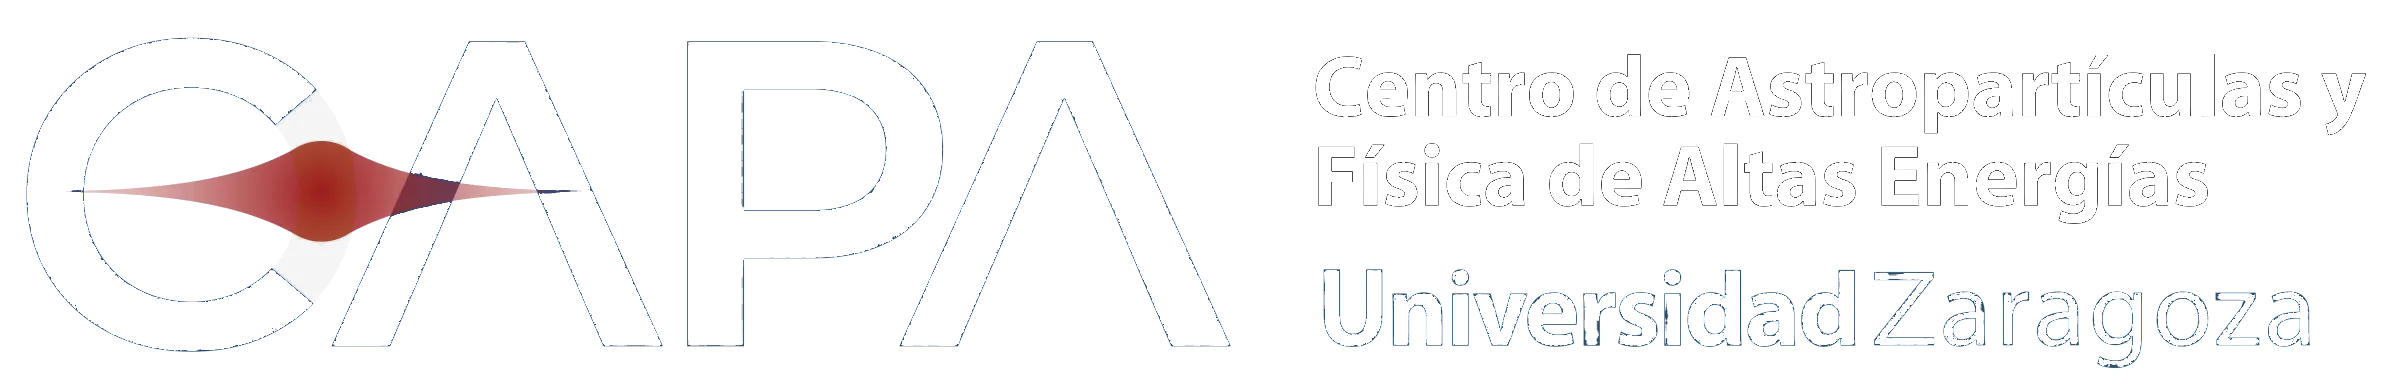
\includegraphics[width=4cm]{logos/CAPA.png}}
\titlepagelogoB{
\includegraphics[width=6cm]{logos/unipd.png}}




\begin{document}
\begin{frame}[noframenumbering,plain]

\titlepage

\end{frame}

\begin{frame}\frametitle{Light New Physics}
    Axion-like Particle coupled to a Peccei-Quinn current of leptons

    $$\mathcal{L}_\mathrm{ALP} = \frac{1}{2}\partial_\mu a \partial^\mu a - \frac{1}{2} m_a^2 a^2 - \frac{1}{2 f_a}\partial_\mu a j^\mu_\mathrm{PQ}\,;$$

    $$j^\mu_\mathrm{PQ} = \sum_{i,j} \left( c_\ell^{ij} \bar{\ell}_i\gamma^\mu \gamma_5 \ell_j + \bar{c}_\ell^{ij} \bar{\ell}_i\gamma^\mu  \ell_j  + c_\nu^{ij} \bar{\nu}_{\ell_i} \gamma^\mu P_L \nu_{\ell_j} \right)\,. $$

    \begin{itemize}
        \item $m_a \in [1\,\mathrm{MeV}, 10\,\mathrm{GeV}]$, $f_a \sim 1\,\mathrm{TeV}$, flavour-universal $c^{ij} = c \delta^{ij}$.
        
        \item $g_\ell = c_\ell m_\ell/f_a$.
        
        \item After integration-by-parts and equations-of-motion
        $$\mathcal{L}_\mathrm{ALP, int} = \sum_\ell \left(i g_\ell \bar{\ell}\gamma_5\ell a + \frac{ig}{2 \sqrt{2} m_\ell} (g_\ell - \bar{g}_\ell + g_{\nu_\ell}) (\bar{\ell}\gamma^\mu P_L \nu_\ell) W^-_\mu a + \mathrm{h.c.} \right) + (V\tilde{V}a)\,.$$

        \item Electroweak-preserving case: $g_\ell - \bar{g}_\ell + g_{\nu_\ell}=0$.
    \end{itemize}
\end{frame}

\begin{frame}\frametitle{Light New Physics}

    Scalar $\phi$ and pseudo-scalar $\hat{\phi}$ bosons:

    $$\mathcal{L}_\mathrm{light NP} \subset \frac{1}{2}\partial_\mu \phi \partial^\mu \phi - \frac{1}{2} m_\phi^2 \phi^2 + \frac{1}{2}\partial_\mu \hat{\phi} \partial^\mu \hat{\phi} - \frac{1}{2} m_{\hat{\phi}}^2 \hat{\phi}^2 - \sum_\ell \bar{\ell}(k_\ell \phi + i \hat{k}_\ell \hat{\phi}\gamma_5) \ell\,.$$

    ~
    
    For the pseudo-scalar boson, we recover the EW-preserving ALP when the couplings are hierarchical $\hat{k}_\ell = g_\ell = c m_\ell/f_a$.
\end{frame}

\begin{frame}\frametitle{Particle decays}
    
    \begin{columns}

        \begin{column}{0.6\textwidth}
            The NP particles can decay to a pair of leptons

            $$\Gamma(S \to \ell^+\ell^-) = \frac{m_S}{8\pi} |K_\ell|^2 \left(1-\frac{4 m_\ell^2}{m_S^2}\right)^{\alpha_S}\,,$$

            {\small with $K_\ell = g_\ell$ and $\alpha_S = 1/2$ for $S=a$, and $K_\ell = k_\ell$ and $\alpha_S = 3/2$ for $S=\phi$.}

            Also decays to $2\gamma$ through a lepton loop.

            ~

            ALPs with $m_a > 2 m_e$ and scalars will typically decay inside the detector.
        \end{column}
        \begin{column}{0.38\textwidth}
            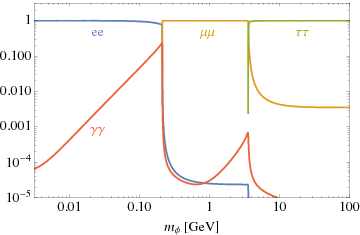
\includegraphics[width=\columnwidth]{figures/BR_S.png} \\
            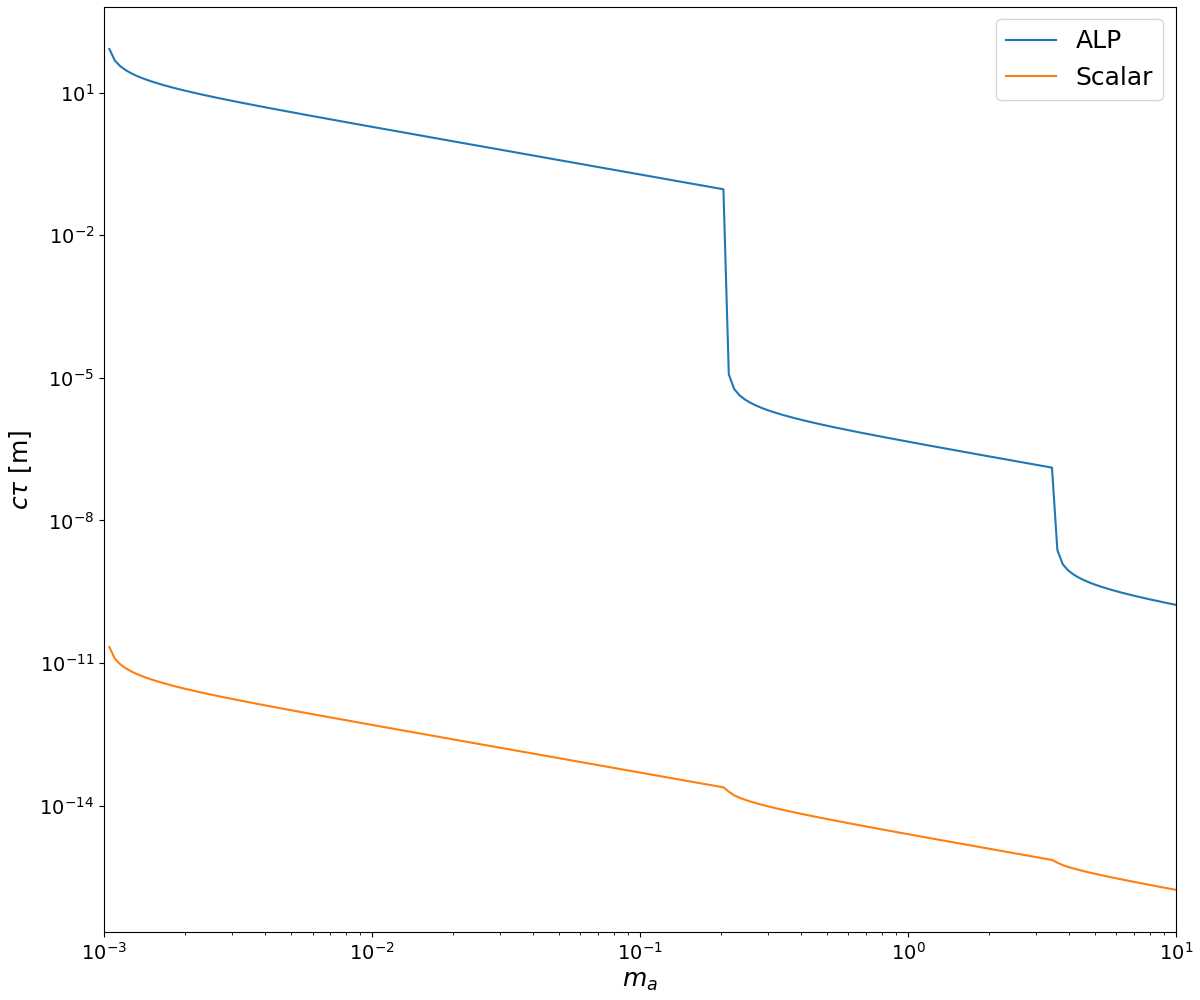
\includegraphics[width=\columnwidth]{figures/properlength.png}
        \end{column}
    \end{columns}
\end{frame}


\end{document}